\documentclass[twoside]{article}
\setlength{\oddsidemargin}{0 in}
\setlength{\evensidemargin}{0 in}
\setlength{\topmargin}{-0.6 in}
\setlength{\textwidth}{6.5 in}
\setlength{\textheight}{8.5 in}
\setlength{\headsep}{0.75 in}
\setlength{\parindent}{0 in}
\setlength{\parskip}{0.1 in}

\usepackage{url}
\usepackage{titlesec}
\setcounter{secnumdepth}{3}
\usepackage{palatino}
\usepackage{marginnote}
\usepackage{multirow}
\usepackage{easybmat,bigdelim,arydshln}
\usepackage[authoryear,round]{natbib}
\usepackage{amssymb,amsmath,amsthm,amsfonts}
\usepackage{mathtools}
%\usepackage{nicematrix}
\usepackage{arydshln}
\usepackage{caption}
\usepackage{hyperref}
\usepackage{tcolorbox}
\tcbuselibrary{skins, breakable, theorems}
\usepackage{newpxtext,newpxmath}
\usepackage{longtable}
\usepackage{enumitem}
\makeatletter

\let\bar\overline

\setlist[itemize]{topsep=0pt,leftmargin=10pt,itemsep=-0.2em}
\usepackage{xcolor}
\usepackage{tikz}
\usepackage{pgfplots}
\pgfplotsset{compat = newest}
\usetikzlibrary{patterns,decorations.pathreplacing,decorations.markings,fit,shapes.geometric,angles,quotes,arrows}
\usepgfplotslibrary{fillbetween}

\usepackage{ifthen}
\usepackage{tikz-3dplot}

\pgfdeclarelayer{ft}
\pgfdeclarelayer{bg}
\pgfsetlayers{bg,main,ft}

\hypersetup{
    colorlinks,
    citecolor=red,
    filecolor=black,
    linkcolor=violet,
    urlcolor=blue
}

\definecolor{myblue}{cmyk}{1,.72,0,.38}
\definecolor{mypurple}{cmyk}{.57,1,0,.58}
\definecolor{myred}{cmyk}{0,.88,.88,.58}
\definecolor{mygreen}{cmyk}{1,0,.69,.66}
\definecolor{myorange}{cmyk}{0,.58,100,.20}
\definecolor{glaucous}{rgb}{0.38, 0.51, 0.71}

\makeatletter
\renewcommand{\thefigure}{\thesection.\arabic{figure}}
\newtheoremstyle{indented}
  {3pt}% space before
  {3pt}% space after
  {\addtolength{\@totalleftmargin}{3.5em}
   \addtolength{\linewidth}{-3.5em}
   \parshape 1 3.5em \linewidth}% body font
  {}% indent
  {\bfseries}% header font
  {.}% punctuation
  {.5em}% after theorem header
  {}% header specification (empty for default)
\makeatother

\newcommand{\ind}{\perp\!\!\!\perp}

\theoremstyle{definition}
\newtheorem{defin}{Definition}[section] % Creates a new counter, number within section
\newtheorem{prt}[defin]{Remark} 
\newtheorem{prts}[defin]{Remarks} % Again share defin's counter
\newtheorem{exmp}[defin]{Example} % etc.
\newtheorem{exmps}[defin]{Examples}
\newtheorem*{note}{Note}
\tcbuselibrary{theorems}

% use counter*=defin to make each tcbtheorem share defin's counter

\newtcbtheorem[use counter*=defin, number within=section]{definition}{Definition}{enhanced, breakable,
    colback = white, colframe = red!55!black, colbacktitle = red!55!black, attach boxed title to top left = {yshift = -2.5mm, xshift = 3mm}, boxed title style = {sharp corners},fonttitle=\bfseries}{def}

\newtcbtheorem[use counter*=defin, number within=section]{theorem}{Theorem}{enhanced, breakable,
    colback = white, colframe = blue!45!black, colbacktitle = blue!45!black, attach boxed title to top left = {yshift = -2.5mm, xshift = 3mm}, boxed title style = {sharp corners},fonttitle=\bfseries}{thm}
    
\newtcbtheorem[use counter*=defin, number within=section]{proposition}{Proposition}{enhanced, breakable,
    colback = white, colframe = teal, colbacktitle = teal, attach boxed title to top left = {yshift = -2.5mm, xshift = 3mm}, boxed title style = {sharp corners},fonttitle=\bfseries}{prop}

\newtcbtheorem[use counter*=defin, number within=section]{lemma}{Lemma}{enhanced, breakable,
    colback = white, colframe = orange!80!black, colbacktitle = orange!80!black, attach boxed title to top left = {yshift = -2.5mm, xshift = 3mm}, boxed title style = {sharp corners},fonttitle=\bfseries}{lemma}

\newtcbtheorem[use counter*=defin, number within=section]{example}{Example}{enhanced, breakable,
    colback = white, colframe = yellow!60!black, colbacktitle = yellow!60!black, attach boxed title to top left = {yshift = -2.5mm, xshift = 3mm}, boxed title style = {sharp corners},fonttitle=\bfseries}{exmp}

\newtcbtheorem[use counter*=defin, number within=section]{assumption}{Assumption}{enhanced, breakable,
    colback = white, colframe = violet!60!white, colbacktitle = violet!60!white, attach boxed title to top left = {yshift = -2.5mm, xshift = 3mm}, boxed title style = {sharp corners},fonttitle=\bfseries}{assump}

\newtcbtheorem[use counter*=defin, number within=section]{algorithm}{Algorithm}{enhanced, breakable,
    colback = white, colframe = green!55!black, colbacktitle = green!55!black, attach boxed title to top left = {yshift = -2.5mm, xshift = 3mm}, boxed title style = {sharp corners},fonttitle=\bfseries}{algm}
%\newtcolorbox{example}[1]{enhanced, breakable, colback = white, colframe = orange!85!black, colbacktitle = orange!85!black, attach boxed title to top left = {yshift = -2.5mm, xshift = 3mm}, boxed title style = {sharp corners},fonttitle=\bfseries, title={Example: #1}}

\newtcbox{\myhl}[1][white]
  {on line, arc = 0pt, outer arc = 0pt,
    colback = #1!20!white, colframe = #1!50!black,
    boxsep = 0pt, left = 1pt, right = 1pt, top = 1pt, bottom = 1pt, boxrule = 0pt, bottomrule =0pt, toprule =0pt}
    
\newtcbox{\myhlrule}[1][white]
  {on line, arc = 0pt, outer arc = 0pt,
    colback = #1!20!white, colframe = #1!50!black,
    boxsep = 0pt, left = 1pt, right = 1pt, top = 1pt, bottom = 1pt, boxrule = 0pt, bottomrule =0.5pt, toprule =0.5pt}
%
% The following commands set up the lecnum (lecture number)
% counter and make various numbering schemes work relative
% to the lecture number.
%
\newcounter{lecnum}
\renewcommand{\thepage}{\thelecnum-\arabic{page}}
\renewcommand{\thesection}{\thelecnum.\arabic{section}}
\renewcommand{\theequation}{\thelecnum.\arabic{equation}}
\renewcommand{\thefigure}{\thelecnum.\arabic{figure}}
\renewcommand{\thetable}{\thelecnum.\arabic{table}}

\newcommand{\sidenotes}[1]{\marginnote{\raggedright\scriptsize#1}}
%
% The following macro is used to generate the header.
%
\newcommand{\lecture}[6]{
   \pagestyle{myheadings}
   \thispagestyle{plain}
   \newpage
   \setcounter{lecnum}{#1}
   \setcounter{page}{1}
   \noindent
   \begin{center}
   \framebox{
      \vbox{\vspace{2mm}
    \hbox to 6.28in { {\bf Econometrics
	\hfill \today} }
       \vspace{4mm}
       \hbox to 6.28in { {\Large \hfill Topic #1: #2  \hfill} }
       \vspace{2mm}
       \hbox to 6.28in { {\it #3 \hfill by #4} }
      \vspace{2mm}}
   }
   \end{center}
   \markboth{Week #1: #2}{Week #1: #2}

   {\bf Key points}: {#5}

   {\bf Disclaimer}: {\it #6}
   \vspace*{4mm}
}
%

\tikzset{-stealth-/.style={decoration={
  markings,
  mark=at position #1 with {\arrow{stealth}}},postaction={decorate}}}

  \tikzset{tangent/.style={
    decoration={
        markings,% switch on markings
        mark=
            at position #1
            with
            {
                \coordinate (tangent point-\pgfkeysvalueof{/pgf/decoration/mark info/sequence number}) at (0pt,0pt);
                \coordinate (tangent unit vector-\pgfkeysvalueof{/pgf/decoration/mark info/sequence number}) at (1,0pt);
                \coordinate (tangent orthogonal unit vector-\pgfkeysvalueof{/pgf/decoration/mark info/sequence number}) at (0pt,1);
            }
    },
    postaction=decorate
},
use tangent/.style={
    shift=(tangent point-#1),
    x=(tangent unit vector-#1),
    y=(tangent orthogonal unit vector-#1)
},
use tangent/.default=1}

\tikzstyle{terminator} = [rectangle, draw, thick, text centered, rounded corners, minimum height=2em]
\tikzstyle{process} = [rectangle, draw, thick, text centered, minimum height=2em]
\tikzstyle{decision} = [diamond, draw, thick, text centered, minimum width=3cm, minimum height=0.5cm]
\tikzstyle{data}=[trapezium, draw, thick, text centered, trapezium left angle=60, trapezium right angle=120, minimum height=2em]
\tikzstyle{arrow} = [thick,->,>=stealth]

\begin{document}
\lecture{16}{Graphical Network Inference}{}{Sai Zhang}{}{The note is built on Prof. \hyperlink{http://faculty.marshall.usc.edu/jinchi-lv/}{Jinchi Lv}'s lectures of the course at USC, DSO 607, High-Dimensional Statistics and Big Data Problems.}
%\footnotetext{These notes are partially based on those of Nigel Mansell.}

\section{Motivation}
Consider a classic question: For $n$ observations of dimension $p$, how can we capture the statistical relationships between the variables of interest? Consider the example of the multivariate Gaussian distribution:
\begin{example}{Multivariate Gaussian Distribution}{}
    Suppose we have $n$ observations of dimension $p$, $\mathbf{x}\sim \mathcal{N}(\boldsymbol{\mu},\boldsymbol{\Sigma})$. let $\mathbf{S}$ be the empirical covariance matrix. Then the probability density 
    $$
    f(\mathbf{x}) = \frac{1}{(2\pi)^{p/2}\det (\boldsymbol{\Sigma})^{1/2}}\exp\left\{ -\frac{1}{2}(\mathbf{x}-\boldsymbol{\mu})'\boldsymbol{\Sigma}^{-1}(\mathbf{x}-\boldsymbol{\mu}) \right\}
    $$
    define the \textbf{inverse covariance matrix} or \textbf{precision matrix} as $ \boldsymbol{\Omega}=\boldsymbol{\Sigma}^{-1} $, then we have 
    $$
    f_{\mathbf{\mu},\boldsymbol{\Omega}} = \exp \left\{ \boldsymbol{\mu'\Omega x} - \left< \boldsymbol{\Omega},\frac{1}{2}\mathbf{xx}' \right> -\frac{p}{2}\log(2\pi) + \frac{1}{2} \log\det(\boldsymbol{\Omega}) - \frac{1}{2}\boldsymbol{\mu'\Omega\mu} \right\}
    $$
    where $\left< \mathbf{A},\mathbf{B} \right> = \mathrm{tr}(\mathbf{AB})$.
\end{example}
In this example, we know that \textbf{every} multivariate Gaussian distribution can be represented by a pairwise \myhl[myblue]{\textbf{Gaussian Markov Random Field (GMRF)}}, which an \textbf{\underline{undirected graph}} $G=(V,E)$
\begin{itemize}
    \item representing the collection of variables $\mathbf{x}$ by a vertex set $\mathcal{V}=\left\{1,\cdots,p\right\}$
    \item encoding correlations between variables by a set of edges $\mathcal{E}=\left\{ (i,j)\in \mathcal{V}\mid i=\neq j,\Omega_{ij}\neq 0 \right\}$  
\end{itemize}

For simplicity, we normalize $\boldsymbol{\mu} = \mathbf{0}$. If we draw $n$ i.i.d. samples $\mathbf{x}_1,\cdots,\mathbf{x}_n \sim \mathcal{N}(\mathbf{0},\boldsymbol{\Sigma})$, then the log-likelihood is
\begin{align*}
    \mathcal{L}(\boldsymbol{\Omega}) &= \frac{1}{n}\sum^n_{i=1}\log f(\mathbf{x}_i) = \frac{1}{2}\log \det (\boldsymbol{\Omega}) - \frac{1}{2n}\sum^n_{i=1}\mathbf{x}'_1\boldsymbol{\Theta}\mathbf{x}_i \\
    &= \frac{1}{2}\log\det (\boldsymbol{\Omega}) - \frac{1}{2}\left< \Omega,\frac{1}{n}\sum^n_{i=1}\mathbf{x}'_i\mathbf{x}'_i \right>
\end{align*}

\paragraph*{What's the goal?} We want to estimate a \myhl[myblue]{\textbf{sparse}} graph structure given $n\ll p$ i.i.d. observations. But what does sparsity means in this context? A sparse graph is \textbf{\underline{equivalent}} to a sparse precision matrix: the precision matrix should have many 0s.

\paragraph*{Sparse precision matrix} for the Gaussian vector mentioned above $\mathbf{x}\sim\mathcal{N}(\mathbf{0},\boldsymbol{\Sigma})$, we have $\forall u,v$ $$ x_u \perp x_v \mid \mathbf{x}_{\mathcal{V}\setminus \left\{ u,v \right\} } \Leftrightarrow \Omega_{u,v}=0 $$
that is, sparsity of the precision matrix is equivalent to \myhl[myblue]{\textbf{conditional independence}}\footnote{Meanwhile, for independence: $\Sigma_{u,v}=0\Leftrightarrow x_u \perp x_v$}. Consider \hyperref[fig:sparse_precision_graph]{a graph}, where $x_1$ and $x_4$ are only connected through other nodes, that is $x_1$ and $x_4$ are conditional independent, then we can have the precision matrix be something like:
$$
\boldsymbol{\Theta} = \begin{bmatrix}
    * & * & 0 & 0 & * & 0 & 0 & 0 \\
    * & * & 0 & 0 & 0 & * & * & 0 \\
    0 & 0 & * & 0 & * & 0 & 0 & * \\
    0 & 0 & 0 & * & 0 & 0 & * & 0 \\
    * & 0 & * & 0 & * & 0 & 0 & * \\
    0 & * & 0 & 0 & 0 & * & 0 & 0 \\
    0 & * & 0 & * & 0 & 0 & * & 0 \\
    0 & 0 & * & 0 & * & 0 & 0 & *
\end{bmatrix}
$$
where 0 captures precisely the conditional independence.

\begin{figure}[ht]\label{fig:sparse_precision_graph}
    \begin{minipage}[b]{0.45\textwidth}
    \centering
    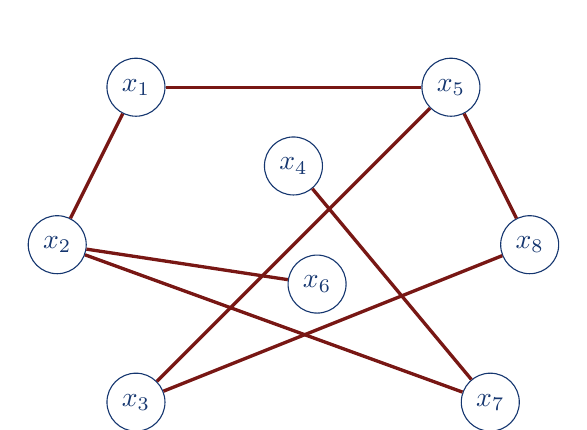
\begin{tikzpicture}[scale=1]
        % Step
        \draw[color=myblue] (-2,4) node[draw,circle] (x1) {$x_1$};
        \draw[color=myblue] (2,4) node[draw,circle] (x5) {$x_5$};
        \draw[color=myblue] (0,3) node[draw,circle] (x4) {$x_4$};
        \draw[color=myblue] (-3,2) node[draw,circle] (x2) {$x_2$};
        \draw[color=myblue] (0.3,1.5) node[draw,circle] (x6) {$x_6$};
        \draw[color=myblue] (3,2) node[draw,circle] (x8) {$x_8$};
        \draw[color=myblue] (-2,0) node[draw,circle] (x3) {$x_3$};
        \draw[color=myblue] (2.5,0) node[draw,circle] (x7) {$x_7$};
        % egdes
        \draw[color=myred, very thick] (x1) -- (x5);
        \draw[color=myred, very thick] (x5) -- (x8);
        \draw[color=myred, very thick] (x8) -- (x3);
        \draw[color=myred, very thick] (x3) -- (x5);
        \draw[color=myred, very thick] (x1) -- (x2);
        \draw[color=myred, very thick] (x2) -- (x6);
        \draw[color=myred, very thick] (x2) -- (x7);
        \draw[color=myred, very thick] (x4) -- (x7);
    \end{tikzpicture}
    
    \textbf{$x_1$ and $x_4$ are \textit{connected}}
    \end{minipage}
    \hfill
    \begin{minipage}[b]{0.45\textwidth}
        \centering
        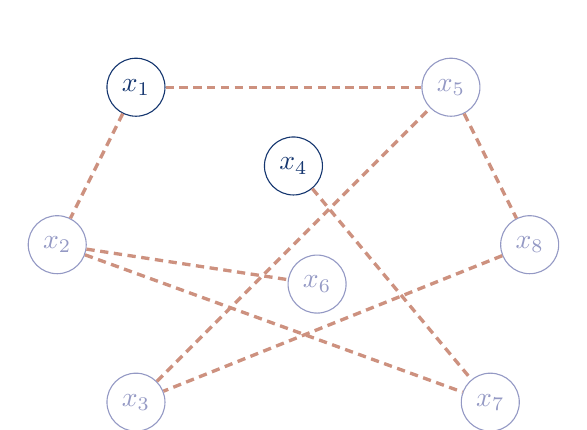
\begin{tikzpicture}[scale=1]
            % Step
            \draw[color=myblue] (-2,4) node[draw,circle] (x1) {$x_1$};
            \draw[color=myblue!35!white] (2,4) node[draw,circle] (x5) {$x_5$};
            \draw[color=myblue] (0,3) node[draw,circle] (x4) {$x_4$};
            \draw[color=myblue!35!white] (-3,2) node[draw,circle] (x2) {$x_2$};
            \draw[color=myblue!35!white] (0.3,1.5) node[draw,circle] (x6) {$x_6$};
            \draw[color=myblue!35!white] (3,2) node[draw,circle] (x8) {$x_8$};
            \draw[color=myblue!35!white] (-2,0) node[draw,circle] (x3) {$x_3$};
            \draw[color=myblue!35!white] (2.5,0) node[draw,circle] (x7) {$x_7$};
            % egdes
            \draw[color=myred!35!white, very thick, densely dashed] (x1) -- (x5);
            \draw[color=myred!35!white, very thick, densely dashed] (x5) -- (x8);
            \draw[color=myred!35!white, very thick, densely dashed] (x8) -- (x3);
            \draw[color=myred!35!white, very thick, densely dashed] (x3) -- (x5);
            \draw[color=myred!35!white, very thick, densely dashed] (x1) -- (x2);
            \draw[color=myred!35!white, very thick, densely dashed] (x2) -- (x6);
            \draw[color=myred!35!white, very thick, densely dashed] (x2) -- (x7);
            \draw[color=myred!35!white, very thick, densely dashed] (x4) -- (x7);
        \end{tikzpicture}
        
        \textbf{$x_1$ and $x_4$ are \textit{NOT connected}, conditionally}
        
    \end{minipage}
\end{figure}

Intuitively, a sparse graph is much simpler, which is why conditional independence is desired. So how to achieve sparsity? We can again use a L-1 regularization when maximizing the log-likelihood $\mathcal{L}(\boldsymbol{\Omega})$. Denote the sample covariance matrix as $\mathbf{S} = \frac{1}{n}\sum^n_{i=1}\mathbf{x}_i\mathbf{x}_i'$, then the problem becomes the so-called \myhl[myblue]{\textbf{Graphical Lasso}}
$$
\max_{\boldsymbol{\Omega}\geq \mathbf{0}}\log \det (\boldsymbol{\Omega}) - \mathrm{tr}(\mathbf{S}\boldsymbol{\Omega}) - \rho\left\Vert \boldsymbol{\Omega} \right\Vert _1
$$
which is equivalent to 
$$
\min_{\boldsymbol{\Omega}\geq \mathbf{0}} -\log \det (\boldsymbol{\Omega}) + \mathrm{tr}(\mathbf{S}\boldsymbol{\Omega}) +\rho\left\Vert \boldsymbol{\Omega} \right\Vert _1
$$

\section{Graphical Lasso}
The graphical lasso method is developed by \citep{friedman2008sparse}. For the optimization problem 
\begin{equation}
    \min_{\boldsymbol{\Omega}\geq \mathbf{0}} -\log \det (\boldsymbol{\Omega}) + \mathrm{tr}(\mathbf{S}\boldsymbol{\Omega}) +\rho\left\Vert \boldsymbol{\Omega} \right\Vert _1 
\end{equation}
The first-order optimality condition gives
\begin{align*}
    &\mathbf{0} \in \boldsymbol{\Omega}^{-1} - \mathbf{S} -\lambda \boldsymbol{\Gamma}
    %\Rightarrow & \boldsymbol{\Omega}^{-1}_{i,i} = \mathbf{S}_{i,i} + \lambda, \ 1\leq i \leq p & \text{in diagonal entries (self-loop), }1\in\partial\left\vert \boldsymbol{\Omega}_{i,i} \right\vert
\end{align*}
where $\boldsymbol{\Gamma}$ is a matrix of component-wise signs of $\boldsymbol{\Omega}$
\begin{align*}
    \boldsymbol{\Gamma} = \partial \left\Vert \boldsymbol{\Omega} \right\Vert _1 & \Rightarrow \gamma_{jk} \begin{cases}
        = \text{sign}(\omega_{jk}), &\omega_{jk}\neq 0\\
        \in  [-1,1], &\omega_{jk}=0
    \end{cases}
\end{align*}
since in a graph, we always have that, following the global stationary conditions, $\omega_{jj}>0$, which implies that 
\begin{align}\label{eq:ghlasso_stationary_condition}
    w_{ii} &= s_{ii} + \lambda & i=1,\cdots,p
\end{align}
where we denote a working version of $\boldsymbol{\Omega}^{-1}$ as $\mathbf{W}$.

The idea is to repeatedly cycle through all columns-rows and in each step optimize only a single column-row. Consider the following partition where all matrices are partitioned into one column/row versus the rest
\begin{align*}
    \boldsymbol{\Omega} &= \begin{pmatrix}
        \boldsymbol{\Omega}_{11} & \boldsymbol{\omega}_{12}\\
        \boldsymbol{\omega}_{12}' & \omega_{22}
     \end{pmatrix} & \mathbf{S} &= \begin{pmatrix}
        \mathbf{S}_{11} & \mathbf{s}_{12}\\
        \mathbf{s}_{12}' & s_{22}
     \end{pmatrix} & \mathbf{W} &= \begin{pmatrix}
        \mathbf{W}_{11} & \mathbf{w}_{12}\\
        \mathbf{w}_{12}' & w_{22}
     \end{pmatrix} & \boldsymbol{\Gamma} &= \begin{pmatrix}
        \boldsymbol{\Gamma}_{11} & \boldsymbol{\gamma}_{12}\\
        \boldsymbol{\gamma}_{12}' & \gamma_{22}
     \end{pmatrix}
\end{align*}
apply this partition to the optimality condition, get
\begin{align*}
    \boldsymbol{\Omega}^{-1} &= \mathbf{S} - \lambda\boldsymbol{\Gamma} \\
    \begin{pmatrix}
        \mathbf{W}_{11} & \mathbf{w}_{12}\\
        \mathbf{w}_{12}' & w_{22}
    \end{pmatrix} &= \begin{pmatrix}
        \mathbf{S}_{11} & \mathbf{s}_{12}\\
        \mathbf{s}_{12}' & s_{22}
     \end{pmatrix} + \lambda \begin{pmatrix}
        \boldsymbol{\Gamma}_{11} & \boldsymbol{\gamma}_{12}\\
        \boldsymbol{\gamma}_{12}' & \gamma_{22}
     \end{pmatrix}
\end{align*}
where $\boldsymbol{\Omega}_{11}$ is $(p-1)\times(p-1)$, $\boldsymbol{\omega}_{12}$ is $(p-1)\times 1$, $\omega_{22}$ is a scalar.

Consider a \myhl[myblue]{\textbf{blockwise}} step: suppose we fix all but the last row/column, then using properties of inverses of block-partitioned matrices, we have 
\begin{align*}
    \begin{pmatrix}
        \mathbf{W}_{11} & \mathbf{w}_{12}\\
        \mathbf{w}_{12}' & w_{22}
     \end{pmatrix} &= \begin{pmatrix}
        \left( \boldsymbol{\Omega}_{11}-\frac{\boldsymbol{\omega}_{12}\boldsymbol{\omega}_{12}'}{\omega_{22}} \right)^{-1} & -\mathbf{W}_{11}\frac{\boldsymbol{\omega}_{12}}{\omega_{22}}\\
         & \frac{1}{\omega_{22}}-\frac{\boldsymbol{\omega}_{12}'\mathbf{W}_{11}\boldsymbol{\omega}_{12}}{\omega^2_{22}}
     \end{pmatrix}\\
     &= \begin{pmatrix}
        \boldsymbol{\Omega}^{-1}_{11}+\frac{\boldsymbol{\Omega}^{-1}_{11}\boldsymbol{\omega}_{12}\boldsymbol{\omega}_{12}'\boldsymbol{\Omega}^{-1}_{11}}{\omega_{22}-\boldsymbol{\omega}_{12}'\boldsymbol{\Omega}^{-1}_{11}\boldsymbol{\omega}_{12}} & -\frac{\boldsymbol{\Omega}^{-1}_{11}\boldsymbol{\omega}_{12}}{\omega_{22}-\boldsymbol{\omega}_{12}'\boldsymbol{\Omega}^{-1}_{11}\boldsymbol{\omega}_{12}} \\
        & \frac{1}{\omega_{22}-\boldsymbol{\omega}_{12}'\boldsymbol{\Omega}^{-1}_{11}\boldsymbol{\omega}_{12}}
     \end{pmatrix}
\end{align*}

then, by the partitioned optimality condition, we have\footnote{For Eq.\ref{eq:modified_glasso_conditions}, by Eq.\ref{eq:ghlasso_stationary_condition}, we know that $w_{22}=s_{22}+\lambda$, which is fixed.}:
\begin{align}\label{eq:glasso_conditions}
    \mathbf{0} &= -\mathbf{w}_{12} + \mathbf{s}_{12}+\lambda \boldsymbol{\gamma}_{12} = \mathbf{W}_{11}\frac{\boldsymbol{\omega}_{12}}{\omega_{22}}+ \mathbf{s}_{12}+\lambda \boldsymbol{\gamma}_{12}
\end{align}
\begin{align}\label{eq:modified_glasso_conditions}
    \mathbf{0} &= \frac{\boldsymbol{\Omega}^{-1}_{11}\boldsymbol{\omega}_{12}}{\omega_{22}-\boldsymbol{\omega}_{12}'\boldsymbol{\Omega}^{-1}_{11}\boldsymbol{\omega}_{12}} + \mathbf{s}_{12} + \lambda\boldsymbol{\gamma}_{12} = w_{22}\boldsymbol{\Omega}^{-1}_{11}\boldsymbol{\omega}_{12} + \mathbf{s}_{12} + \lambda\boldsymbol{\gamma}_{12}
\end{align}

The graphic Lasso algorithm them solves Eq.\ref{eq:glasso_conditions} for $\boldsymbol{\beta}=\boldsymbol{\omega}_{12}/\omega_{12}$, that is
$$
\mathbf{W}_{11}\boldsymbol{\beta} + \mathbf{s}_{12} + \lambda\boldsymbol{\gamma}_{12} = \mathbf{0}
$$
where $\boldsymbol{\gamma}_{12}\in\mathrm{sign}(\boldsymbol{\beta})$ since $\omega_{22}>0$, which is essentially solving:
$$
\min_{\boldsymbol{\beta}\in\mathbb{R}^{p-1}}\left\{ \frac{1}{2}\boldsymbol{\beta}'\mathbf{W}_{11}\boldsymbol{\beta} + \boldsymbol{\beta}'\mathbf{s}_{12} + \lambda\left\Vert \boldsymbol{\beta} \right\Vert _1 \right\}
$$
and $\mathbf{W}_{11}>0$ is assumed to be fixed. 

This problem is analogous to a lasso regression problem of \myhl[myblue]{the \textbf{last variable} on \textbf{the rest}}, but the cross-product matrix $\mathbf{S}_{11}$ is replaced by its \textbf{\underline{current estimation}} $\mathbf{W}_{11}$. It is relatively easier to solve using elementwise coordinate descent, then
\begin{align*}
    \mathbf{w}_{12} &= -\mathbf{W}_{11}\frac{\boldsymbol{\omega}_{12}}{\omega_{22}} &\Rightarrow \hat{\mathbf{w}}_{12} &= -\mathbf{W}_{11}\hat{\boldsymbol{\beta}} & \text{Step 1}\\
    w_{22} &= \frac{1}{\omega_{22}}-\frac{\boldsymbol{\omega}_{12}'\mathbf{W}_{11}\boldsymbol{\omega}_{12}}{\omega^2_{22}} &\Rightarrow \frac{1}{\hat{\omega}_{22}} &= w_{22} - \hat{\boldsymbol{\beta}}'\hat{\mathbf{w}}_{12} & \text{Step 2} \\
    \boldsymbol{\omega}_{12} &= -\mathbf{W}_{11}^{-1}\mathbf{w}_{12}\omega_{22} &\Rightarrow \hat{\boldsymbol{\omega}}_{12} &= -\mathbf{W}^{-1}_{11}\hat{\mathbf{w}}_{12}\hat{\omega}_{22} & \text{Step 3}
\end{align*}
notice that after solving for $\boldsymbol{\beta}$ and updating $\mathbf{w}_{12}$ in Step 1, the graphic Lasso procedure can move onto the next block, that is, only Step 1 is used in the loop, Step 2 and 3 can be done at the end. The algorithm can be summarized as:

\begin{algorithm}{Graphical Lasso algorithm}{glasso_algorithm}
    \begin{itemize}
        \item[1] Initialize $\mathbf{W}= \mathbf{S} + \lambda\mathbf{I}$ 
        \item Cycle around the columns repeatedly, performing the following steps till convergence: 
        \begin{itemize}
            \item[a] rearrange the rows/columns so that the target column is \textbf{\underline{the last}} (implicitly)
            \item[b] solve the lasso problem, starting the solution from the previous round for this column
            \item[c] update the row/column (\textbf{\textit{off-diagonal}}) of the covariance using $\hat{\mathbf{w}}_{12}$
            \item[d] save $\hat{\boldsymbol{\beta}}$ for this column in the matrix $\mathbf{B}$
        \end{itemize}
        \item[3] after convergence, for every row/column, compute the diagonal entries $\hat{\omega}_{jj}$, and covert the $\mathbf{B}$ matrix to $\boldsymbol{\Omega}$
    \end{itemize}
\end{algorithm}

\paragraph*{Issues of GLasso method}:
\begin{itemize}
    \item $\boldsymbol{\theta}_{12}$ is entangled in $\mathbf{W}_{11}$, which is \myhl[myblue]{\textbf{\textit{incorrectly}}} treated as a constant
    \item after updating $\boldsymbol{\theta}_{12}$, the entire (working) covariance matrix $\mathbf{W}$ changes, but Glasso algorithm only updates $\mathbf{w}_{12}$ and $\mathbf{w}_{12}'$
\end{itemize}
Together, the two issues lead to the non-monotonic behavior of Glasso in minimizing $f(\boldsymbol{\Omega})$. Next, we address these issues by introducing some modifications.

\section{Graphical Lasso: Modifications}
Consider the optimality condition in Eq.\ref{eq:modified_glasso_conditions}:
\begin{align*}
    \mathbf{0} &= \frac{\boldsymbol{\Omega}^{-1}_{11}\boldsymbol{\omega}_{12}}{\omega_{22}-\boldsymbol{\omega}_{12}'\boldsymbol{\Omega}^{-1}_{11}\boldsymbol{\omega}_{12}} + \mathbf{s}_{12} + \lambda\boldsymbol{\gamma}_{12} = w_{22}\boldsymbol{\Omega}^{-1}_{11}\boldsymbol{\omega}_{12} + \mathbf{s}_{12} + \lambda\boldsymbol{\gamma}_{12}
\end{align*}
Here, the dependence of the covariance submatrix $\mathbf{W}_{11}$ on $\boldsymbol{\Omega}_{12}$ is \myhl[myblue]{\textbf{explicit}}. Let $\boldsymbol{\alpha} = \boldsymbol{\omega}_{12}w_{22}$ with fixed $w_{22}\geq 0$\footnote{$w_{22}= 1/(\omega_22-\boldsymbol{\omega}_{12}'\boldsymbol{\Omega}_{11}^{-1}\boldsymbol{\omega}_{12})$}, then this optimality condition is essentially solving
$$
\min_{\boldsymbol{\alpha}\in\mathbb{R}^{p-1}}\left\{ \frac{1}{2}\boldsymbol{\alpha'\Omega}_{11}^{-1}\boldsymbol{\alpha} + \boldsymbol{\alpha}'\mathbf{s}_{12} + \lambda\left\Vert \boldsymbol{\alpha}\right\Vert _1 \right\}
$$
the minimizer of this problem $\hat{\boldsymbol{\alpha}}$ can then be used to derive the estimation for $\boldsymbol{\omega}_{12}$: $$\hat{\boldsymbol{\omega}}_{12} = \frac{\hat{\boldsymbol{\alpha}}}{w_{22}}$$, then we can update $\omega_{22}$ as before via $$ \hat{\omega}_{22} = \frac{1}{w_{22}} + \hat{\boldsymbol{\omega}}_{12}'\boldsymbol{\Theta}^{-1}_{11} \hat{\boldsymbol{\omega}}_{12}$$ with $w_{22}=s_{22}+\lambda$. Another problem is how to obtain $\boldsymbol{\Omega}^{-1}_{11}$: as the iterations proceed, maintain $\mathbf{W}=\boldsymbol{\Omega}^{-1}$, and $\boldsymbol{\Omega}^{-1}_{11}$ can be derived from $$ \boldsymbol{\Omega}^{-1}_{11}=\mathbf{W}_{11}-\frac{\mathbf{w}_{12}\mathbf{w}_{12}'}{w_{22}} $$
once $\boldsymbol{\omega}_{12}$ is updated, the \myhl[myblue]{\textbf{\textit{entire}}} working covariance matrix $\mathbf{W}$ is updated using $\boldsymbol{\Omega}^{-1}_{11}$. This procedure, the so-called primal graphical lasso, can be represented in the following algorithm:

\begin{algorithm}{P-GLasso Algorithm}{pglasso_algorithm}
    \begin{itemize}
        \item[1] Initialize $\mathbf{W} = \mathrm{diag}(\mathbf{S}) + \lambda\mathbf{I}$ and $\boldsymbol{\Omega} = \mathbf{W}^{-1}$
        \item[2] Cycle around the columns repeatedly, performing the following steps till convergence:
        \begin{itemize}
            \item[a] rearrange the rows/columns so that the target column is the last (implicitly)
            \item[b] compute $\mathbf{\Omega}^{-1}_{11}$ using $\boldsymbol{\Omega}^{-1}_{11}=\mathbf{W}_{11}-\frac{\mathbf{w}_{12}\mathbf{w}_{12}'}{w_{22}}$
            \item[c] solve $\min_{\boldsymbol{\alpha}\in\mathbb{R}^{p-1}}\left\{ \frac{1}{2}\boldsymbol{\alpha'\Omega}_{11}^{-1}\boldsymbol{\alpha} + \boldsymbol{\alpha}'\mathbf{s}_{12} + \lambda\left\Vert \boldsymbol{\alpha}\right\Vert _1 \right\} $ for $\boldsymbol{\alpha}$, using as warm starts the solution from the previous round of row/column updates. Then update $\hat{\boldsymbol{\omega}_{12}} = \hat{\boldsymbol{\alpha}}/w_{22}$ and $\hat{\omega_{22}}$
            \item[d] update $\boldsymbol{\Omega}$ and $\mathbf{W}$, ensuring that $\boldsymbol{\Omega}\mathbf{W} = \mathbf{I}_p$
        \end{itemize}
        \item[3] d
    \end{itemize}
\end{algorithm}


\newpage
\bibliographystyle{plainnat}
\bibliography{ref.bib}

\end{document}